\documentclass{article}

\usepackage[margin=0.5in]{geometry}
\usepackage{multicol}
\usepackage{graphicx}

\title{Problem-Solving Set B}
\author{}
\date{}

\begin{document}
\maketitle
\noindent Problems should be solved without a calculator unless otherwise specified.
Remember to explain how you solved a problem.
\begin{multicols}{2}
    \begin{enumerate}
        \item What is the degree measure of angle $A$?
            \begin{center}
                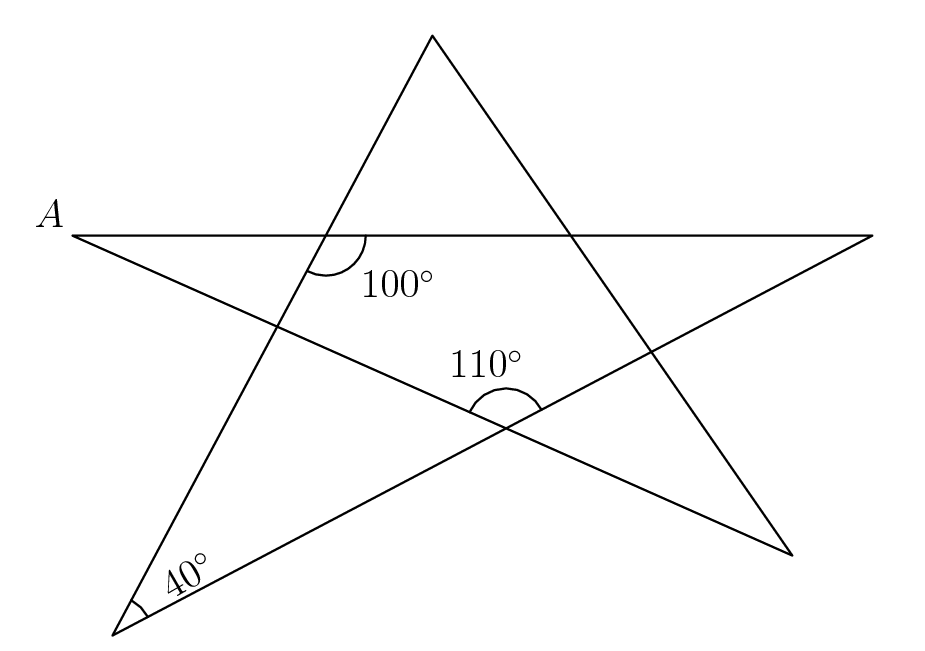
\includegraphics[scale=0.15]{star.png}
            \end{center}
            \vspace{3cm}
        \item What is the remainder of $1999^{2000}$ when it is divided by $5$?
            \vspace{3cm}
        \item Harold tosses a nickel four times.
            What is the probability that he gets at least as many heads as tails?
            \vspace{3cm}
        \item Loki, Moe, Nick, and Ott are good friends.
            Ott had no money, but the others did.
            Moe gave Ott one-fifth of his money, Loki gave Ott one-fourth of his money, and Nick gave Ott one-third of his money.
            Each gave Ott the same amount of money.
            What fractional part of the group's money does Ott have now?
            \vspace{3cm}
        \item Bicycle license plats in Flatville each contain three letters.
            The first is chosen from the set $\{C,H,L,P,R\}$, the second from $\{A,I,O\}$, and the third from $\{D,M,N,T\}$.
            When Flatville needed more license plates, they added two new letters, The new letters may both be added to one set or one letter may be added to one set and one to another set.
            What is the largest possible number of ADDITIONAL license plates that can be made by adding two letters?
            \vspace{3cm}
    \end{enumerate}
\end{multicols}
\end{document}